\documentclass[10pt,a4paper,]{report}
\usepackage[french]{babel}
\usepackage{amsfonts}
\usepackage{amsmath}
\usepackage{shapepar}
\usepackage{amssymb}
\usepackage{latexsym}
\usepackage{makeidx}
\usepackage{color}
\usepackage{verbatim}
\usepackage{fancyhdr}
\usepackage{setspace}
\usepackage{amsmath}
\usepackage{amssymb}
\usepackage{latexsym}
\usepackage{graphicx}
\usepackage{collcell}
\usepackage{lettrine}
\usepackage{listings}
\newcommand{\includepic}[1]{\includegraphics[width=8cm,
	height=8cm, keepaspectratio]{#1}}
\newcolumntype{i}{@{\hspace{1ex}}
	>{\collectcell\includepic}c<{\endcollectcell}}
\usepackage{makeidx}
\usepackage{color}
\usepackage{fancyhdr}
\usepackage{bbm}
\usepackage{bbold}
\usepackage{babel}
\usepackage{setspace}
\usepackage{fancybox}
\usepackage[utf8]{inputenc}
\usepackage{amsthm}
\usepackage[french]{babel}
\usepackage[dvips, lmargin=2.5cm, rmargin=2.5cm, tmargin=3.5cm, bmargin=3cm]{geometry}
\usepackage{fancyhdr}
\usepackage[listing]

\newcounter {subsubsubsection}[subsubsection]
\setcounter{secnumdepth}{4}
\setcounter{tocdepth}{4}
\newtheorem{Th}{\sc \bf Theorem}[section]
\newtheorem{thm}[Th]{\bf Théor\`eme}
\newtheorem{cor}[Th]{\bf Corollory}
\newtheorem{lem}[Th]{\bf Lemme}
\newtheorem{prop}[Th]{\bf Proposition}
\newtheorem{notat}[Th]{ Notation}
\newtheorem{nota}[Th]{}
\newtheorem{notatDef}[Th]{ Notation et Définition}
\newtheorem{Def}[Th]{\bf Définition}
\newtheorem{Defs}[Th]{\bf Définitions}
\newtheorem{defprop}[Th]{\bf Proposition et Définition}
\newtheorem{thd}[Th]{\bf Théorème et Définitions}
\newtheorem{Dep}[Th]{\bf  Définitions  et propriétés}
\newtheorem{rem}[Th]{ Remarque}
\newtheorem{rems}[Th]{ Remarques}
\newtheorem{ex}[Th]{ Exemple}
\newtheorem{exs}[Th]{ Exemples}
%\newtheorem{Q}[Th]{\bf Question}
\newtheorem{dfn}[Th]{\bf Définitions}
\newtheorem{nots}{\bf Notes}
\newcommand{\pr} { Preuve }
\newcommand{\dem} { {\bf Démonstration} }
\newcommand{\co} {{ Conclusion   }}
\newcommand{\ra} {{ Rappel   }}
\newtheorem{exe}[Th]{ Exercice}
\newtheorem{exes}[Th]{ Exercices}
\newtheorem{con}[Th]{ conséquence}
\newtheorem{Not}[Th]{ Notations et remarques}
\newtheorem{abs}[Th]{\bf Abstract}
\newtheorem{Nota}[Th]{ Notations}
\newtheorem{propr}[Th]{ Propriétés}
%%%%%%%%%%%%%%%%%%%%%%%%%%%%%%%%%%%%%%%%%%%%%%%%%%%%%%%%%
%%%%%%%%%%%%%%%%%%%%%%%%%%%%%%%%%%%%%%%%%%%%%%%%%%%%%%%%%
\newcommand{\MAT}{$$
	\left(
	\begin{array}}
\newcommand{\mat}{\end{array}
	\right)
	$$}
%%%%%%%%%%%%%%%%%%%%%%%%%%%%%%%%%%%%%%%%%%%%%%%%%%%%%%%%%
\renewcommand{\thefootnote}{\arabic{footnote}}
\newcommand{\ga}{{\mathfrak{a}}}
\newcommand{\gm}{{\mathfrak{m}}}
\newcommand{\argmin}{\operatornamewithlimits{argmin}}
\newcommand{\argmax}{\operatornamewithlimits{argmax}}
%%%%%%%%%%%%%%%%%%%%%%%%%%%%%%%%%%%%%%%%%%%%%%%%%%%%%%%%%
\def\Proof{{\parindent0pt {\bf Proof.\ }}}
%%%%%%%%%%%%%%%%%%%%%%%%%%%%%%%%%%%%%%%%%%%%%%%%%%%%%%%%%
\newcommand{\field}[1]{\mathbb{#1}}
\newcommand{\C}{\field{C}}
\newcommand{\R}{\field{R}}
\newcommand{\Z }{\field{Z}}
\newcommand{\N }{\field{N}}
\newcommand{\K}{\field{K}}
\newcommand{\F }{\field{F}}
\newcommand{\Q}{\field{Q}}
\newcommand{\gp}{{\mathfrak{p}}}
\newcommand{\overbar}[1]{\mkern 1.5mu\overline{\mkern-1.5mu#1\mkern-1mu}\mkern 1mu}
\def\PP{I\!\! P}
%%%%%%%%%%%%%%%%%%%%%%%%%%%%%%%%%%%%%%%%%%%%%%%%%%%%%%%%%
\def\Ext{{\rm Ext}}
\def\Tor{{\rm Tor}}
\def\dim{{\rm dim}}
\def\g{{\rm G-dim}}
\def\wdim{{\rm wdim}}
\def\gldim{{\rm gldim}}
\def\sup{{\rm sup}}
\def\inf{{\rm inf}}
\def\qf{{\rm qf}}
\def\Im{{\rm Im}}
\def\Coker{{\rm Coker}}
\def\Ker{{\rm Ker}}
\def\beq{\begin{eqnarray*}}
	\def\eeq{\end{eqnarray*}}
\def\htt{{\rm ht}}
\def\max{{\rm max}}
\def\Spec{{\rm Spec}}
\def\pd{{\rm pd}}
\def\fd{{\rm fd}}
\def\id{{\rm id}}
%%%%%%%%%%%%%%%%%%%%%%%%%%%%%%%%%%%%%%%%%%%%%%%%%%%%%%%%%
\def\Rom #1{\uppercase\expandafter{\romannumeral #1}}
%%%%%%%%%%%%%%%%%%%%%%%%%%%%%%%%%%%%%%%%%%%%%%%%%%%%%%%%%
\newcommand{\cqfd}
{\hspace{0.5cm}
	\rule{2mm}{2mm}%
	\medbreak%
	\par%
}
%%%%%%%%%%%%%%%%%%%%%%%%%%%%%%%%%%%%%%%%%%%%%%%%%%%%%%%%%
\usepackage[colorlinks, hyperindex, bookmarks, linkcolor=blue, citecolor=blue, urlcolor=blue]{hyperref}

\footskip = 60 pt
\begin{document}
	\includegraphics[height=2.5cm]{facultdescien.png} \hfill{\includegraphics[height=2.5cm]{téléchargement.png}}
	\\
	\\
	\begin{center}
		Université de Montpellier\\
		Faculté des Sciences \\
		\vspace*{2.0cm}
		
		\textbf{PROJET HMMA307 }\\
		\vspace{1.5cm}
		
		Spécialité : \textsl{MIND/SIAD} \\
		\vspace{1.5cm}
		Etudiant :\\
	
		\textit{\textbf{ Cherif AMGHAR}}\\
		\vspace*{3cm} 
		Sous le thème 
		\rule{16cm}{4pt}\\
		\begin{cursive}
			\textcolor{blue}{\textbf{\textit{\Large{Modèles mixtes linéaires}}}} 
		\end{cursive}
		\rule{14cm}{3pt}\\
		\vspace*{1.5cm}
		Enseignant: 
		\vspace*{1.5cm}
		$$
		\begin{array}{lll}

        \textit{\textbf{Pr.  Joseph Salmon  }}
	    \end{array}
		$$
		
		
		\vspace*{1cm}
		08 Novembre 2020
	\end{center}
    \newpage

\begin{spacing}{1}

\tableofcontents

\pagestyle{fancy}
\renewcommand{\footrulewidth}{2pt}
\fancyhf{}
\fancyfoot[L]{ \textit{\texttt{Projet HMMA307} $2020$}}
\fancyfoot[C]{\thepage}
\fancyfoot[R]{\texttt{AMGHAR Cherif}}

\renewcommand{\headrulewidth}{2pt}
\fancyhead[C]{{\rightmark}}
\newpage
\chapter*{Introduction}
\addcontentsline{toc}{chapter}{Introduction}
Un modèle linéaire mixte est un modèle pour lequel le modèle comprend à la fois des effets fixes et des
effets aléatoires. Les MLM incluent des variables à effets fixes et aléatoires. Le mélange entre les deux est à
l'origine du nom. Les effets fixes décrivent les relations entre les covariables et la variable dépendante pour
une population entière, les effets aléatoires sont spécifiques à l'échantillon.\\
En d'autres termes, un effet aléatoire est un effet dont nous ne voulons pas généraliser les propriétés (les
modalités ont été choisies de manière aléatoire dans quelque chose de plus grand) et un effet fixe est un
effet dont on veut généraliser les propriétés. Il s'agit de la variable manipulée dont nous avons choisi les
niveaux spécifiques.


Les données qu'on analyse ici sont des dénombrements d'invertébrés sur 3-4 sites dans chacun des 7 estuaires (choisis au hasard). Ici, les estuaires sont l'effet aléatoire, car il existe un grand nombre d'estuaires possibles, et on n'échantillonne que quelques-uns d'entre eux au hasard, mais on aime faire des inférences sur les estuaires en général.\\
Tout au long de ce projet, on s'intéresse à deux  principaux types de modèles linéaires mixtes, modèle mixtes à un effets aléatoires et le deuxième pour deux effets aléatoires, on explique les sorties sous python.

\newpage
\chapter{Modèles mixtes linéaires avec un effet aléatoire }
 On analyse un ensemble de données visant à tester l'effet de la pollution de l'eau sur l'abondance de certains invertébrés marins subtidaux en comparant des échantillons d'estuaires modifiés et vierges. Comme le nombre total est important, on suppose que les données sont continues.
\\
Modèles mixtes à un effet aléatoire est une introduction aux modèles mixtes pour une réponse continue avec un effet aléatoire . On apprend à vérifier les hypothèses et à faire des inférences, y compris le bootstrap paramétrique.\\
l'équation du modèle est: $$y_{ij} = \beta_0 + u_{0i} + \beta_1 \times t_{ij} + \varepsilon_{ij}$$


$ i $ indexe les individus et $ j $ indexe les variables(modification, estuaries, site, hydriod,..) . Ainsi, $ i \in  \llbracket 1 ,...,54 \rrbracket $ et $ j \in  \llbracket 1,..,6 \rrbracket . $


\section{Propriétés des modèles mixtes}
Les modèles mixtes font des hypothèses importantes:\\
1. (y|x) sont i.i.d et suit loi normale\
2. V(y|x) est constante\\
3. y s'écrit sous forme linéaire en fonction de x et z(l'effet aléatoire) .\\
4. y est indépendant de z\\
5. z suit loi normale.\\

Il est important de vérifier que nos données répondent aux hypothèses du modèle qu'on a utilisé. on regarde toutes les hypothèses dans l'ordre.
\section{Ajustement du modèle: un effet fixe et aléatoire}
Dans cet ensemble de données, hypothèses vérifiés, on a un effet fixe (Modification; modifié vs vierge) et un effet aléatoire (Estuaire). Pour ajuster un modèle d'abondance totale. On ajuste le modèle complet par maximum de vraisemblance, et un deuxième modèle qui n'a pas l'effet fixe de Modification. On obtient que l'effet fixe c'est à dire l'effet de modification permet d'affecter sur le modèle et que le modèle qui contient la plus petit valeur de AIC est le modèle complet. On compare ces deux modèles avec un test de rapport de vraisemblance.
\begin{center}
    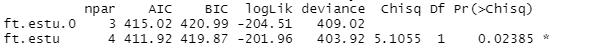
\includegraphics[]{Comparaisonmmod.PNG}
\end{center}
On constate qu'il existe des preuves d'un effet de modification (p = 0,02385).
Et pour tester les variables aléatoires soit on utilise le test d'anova, mais les p-value sont très approximatives, on utilise un bootstrap paramétrique. Il s'agit d'une méthode basée sur la simulation.

\begin{center}
    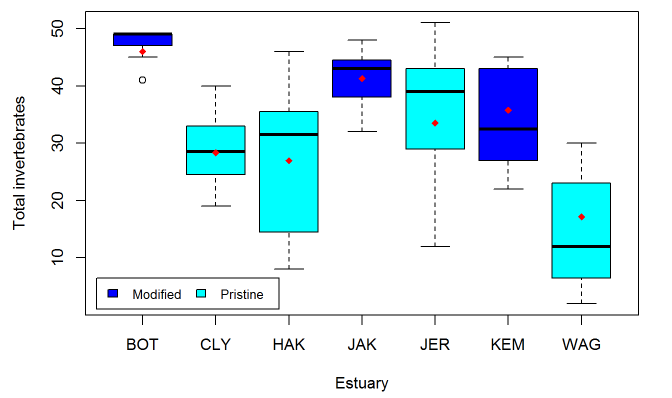
\includegraphics[width=12cm]{resmod1.PNG}
\end{center}
Pour un modèle mixte simple avec un effet aléatoire(Estuary), un graphique des données brutes avec les moyens du modèle superposés est une possibilité de voir les choses.

\chapter{Modèles mixtes linéaires avec des facteurs croisés ou imbriqués }
Deux facteurs sont croisés lorsque chaque catégorie (niveau) d'un facteur coexiste dans la conception avec chaque catégorie de l'autre facteur. En d'autres termes, il y a au moins une observation dans chaque combinaison de catégories pour les deux facteurs.\\
Un facteur est imbriqué dans un autre facteur lorsque chaque catégorie du premier facteur coexiste avec une seule catégorie de l'autre. En d'autres termes, une observation doit être dans une catégorie du facteur 2 pour avoir une catégorie spécifique de facteur 1. Toutes les combinaisons de catégories ne sont pas représentées. Il existe également des plans intermédiaires qui sont partiellement croisés, où certains niveaux d'un facteur se produisent dans plusieurs niveaux (mais pas tous) du deuxième facteur. Ces conceptions ont souvent été enseignées comme des problèmes séparés avec différentes façons d'effectuer des analyses de variance (ANOVA) selon que vous avez des facteurs croisés ou imbriqués.

on analyse un ensemble de données visant à tester l'effet de la pollution de l'eau sur l'abondance de certains invertébrés marins subtidaux en comparant des échantillons d'estuaires modifiés et vierges. Comme le nombre total est important, nous supposerons que les données sont continues.
\section{Ajuster un modèle avec un effet fixe et plusieurs effets aléatoires}
Dans cet ensemble de données, on a un effet fixe (Modification; modifié vs vierge) et deux effets aléatoires (Estuaire et Site). Le site est imbriqué dans l'estuaire car chaque site ne peut appartenir qu'à un seul estuaire. On remarque que l'estuaire JAK et l'estuaire JER ont chacun des sites numérotés 1, même si ces sites ne sont en aucun cas connectés. c'est pour ça on imbrique la variable site dans le Etuary on peut faire cette solution dans le premier temps c'est à dire dans l'étape de saisie de données mais si les choses sont les mêmes elle devraient étiquetées de la même façon et dans le cas inverse elles devraient être différemment.
\section{Vérification des hypothèses}
Les hypothèses sont les mêmes que pour un facteur aléatoire.\\
En bref, les hypothèses 1 et 5 ne peuvent pas être vérifiées, mais peuvent être assurées en prélevant des échantillons aléatoires, et l'hypothèse 6 n'est pas cruciale et difficile à vérifier. Pour vérifier l'hypothèse 2, on recherche une relation en ligne droite sur le graphique des résidus. Pour vérifier les hypothèses 3 et 4, on recherche une forme en éventail et une forme en U sur le tracé résiduel par rapport à l'ajustement. \\
Ajustement avec anova.
\begin{center}
    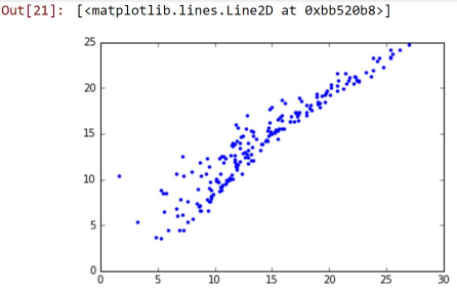
\includegraphics[width=12cm]{plotdon.PNG}
\end{center}
\newpage
Test d'hypothèse pour les effets aléatoires:\\

Comme dans les modèles mixtes 1, on utilise un bootstrap paramétrique. On va tester si on doit avoir un effet aléatoire pour Site étant donné que on a un effet aléatoire pour Estuaire dans le modèle.
\begin{center}
    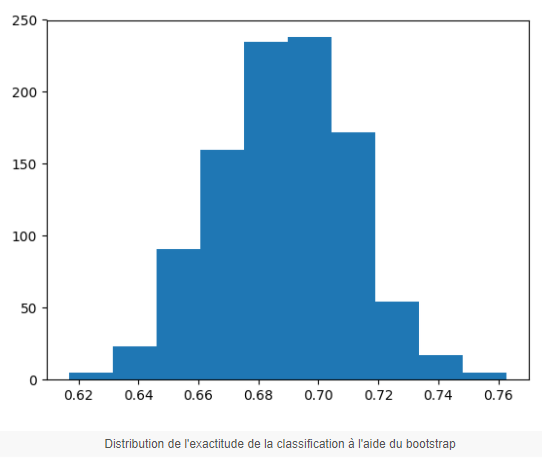
\includegraphics[width=12cm]{distribdonbootstrap.PNG}
\end{center}
les intervalles de confiance sont rapportés, montrant qu'il existe une probabilité de 95(percent) que les intervalles de confiance 64,4(percent) et 73,0(percent) couvrent la véritable compétence du modèle.

On peut interpréter les résultats:en utilisant:


\begin{center}
    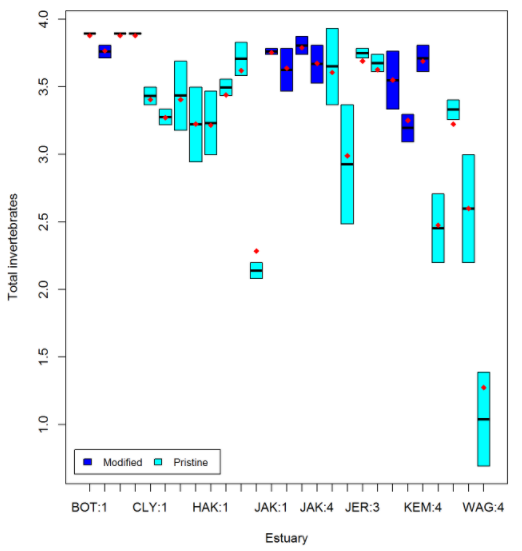
\includegraphics[width=12cm]{rsemod2.PNG}
\end{center}
On peut tracer dans chaque site, mais c'est un peu étrange pour un boxplot car il n'y a que deux observations par site, on peut utiliser si on a  plus d'observations dans chaque site.
\end{document}